% ! TeX program = lualatex
\documentclass[a4paper,11pt]{article} 
% packages
\usepackage{censor}
\StopCensoring
\usepackage{fontspec}
\setmainfont{EB Garamond}
% for tironian et fallback
% % \directlua{luaotfload.add_fallback
% % ("emojifallback",
% %      {"Noto Serif:mode=harf"}
% % )}
% % \setmainfont{EB Garamond}[RawFeature={fallback=emojifallback}]

\setmonofont[Scale=MatchLowercase]{Deja Vu Sans Mono}
\usepackage[a4paper,left=2cm,right=2cm,top=\dimexpr15mm+1.5\baselineskip,bottom=2cm]{geometry}
\setlength{\parindent}{0pt}

\usepackage{fancyhdr}       % Headers and footers 
\fancyhead[R]{\normalfont \leftmark}
\fancyhead[L]{}
\pagestyle{fancy}

\usepackage{microtype}      % Slightly tweak font spacing for aesthetics
\usepackage[english]{babel} % Language hyphenation and typographical rules
\usepackage{xcolor}
\definecolor{linkblue}{RGB}{0, 64, 128}
\usepackage[final, colorlinks = false, urlcolor = linkblue]{hyperref} 
% \newcommand{\secref}[1]{\textbf{§~\nameref{#1}}}
\newcommand{\secref}[1]{\textbf{§\ref{#1}~\nameref{#1}}}

\usepackage{amsmath}
\usepackage[most]{tcolorbox}
\usepackage{changepage}     % adjust margins on the fly
\usepackage{amsmath,amssymb}

\usepackage{minted}
\usemintedstyle{algol_nu}

\usepackage{pgfplots}
\pgfplotsset{width=\textwidth,compat=1.9}

\usepackage{caption}
\newenvironment{code}{\captionsetup{type=listing}}{}
\captionsetup[listing]{skip=0pt}
\setlength{\abovecaptionskip}{5pt}
\setlength{\belowcaptionskip}{5pt}

\usepackage[yyyymmdd]{datetime}
\renewcommand{\dateseparator}{--}

\usepackage{enumitem}

\usepackage{titlesec}

\author{Andrew Hayes}

\begin{document}
\begin{titlepage}
    \begin{center}
        \hrule
        \vspace*{0.6cm}
        \Huge \textsc{cs4423}
        \vspace*{0.6cm}
        \hrule
        \LARGE
       \vspace{0.5cm}
       Networks
       \vspace{0.5cm}
       \hrule

       \vfill

       \hrule
        \begin{minipage}{0.495\textwidth} 
            \vspace{0.4em}
            \raggedright
            \normalsize 
            \begin{tabular}{@{}l l}
                Name: & Andrew Hayes \\
                Student ID: & 21321503 \\
                E-mail: & \href{mailto://a.hayes18@universityofgalway.ie}{a.hayes18@universityofgalway.ie} \\
            \end{tabular}
        \end{minipage}
        \begin{minipage}{0.495\textwidth} 
            \raggedleft
            \vspace*{0.8cm}
            \Large
            \today
            \vspace*{0.6cm}
        \end{minipage}
        \medskip\hrule 
    \end{center}
\end{titlepage}

\pagenumbering{roman}
\newpage
\tableofcontents
\newpage
\setcounter{page}{1}
\pagenumbering{arabic}

\section{Introduction}
\textbf{CS4423 Networks} is a Semester 2 module on \textbf{Network Science}.
Modern societies are in many ways highly connected.
Certain aspects of this phenomenon are frequently described as \textbf{networks}.
CS4423 is an introduction to this emerging interdisciplinary subject.
We'll cover several major topics in this module, including:
\begin{itemize}
    \item   Graphs \& Graph Theory,  and how they relate to networks;
    \item   Representations of networks, including as matrices;
    \item   Computing with networks, using \mintinline{python}{networkx} in Python;
    \item   Centrality measures;
    \item   Random graphs;
    \item   Small worlds;
    \item   Models of growing graphs;
\end{itemize}

Lecture notes \& assignments will come in the form of Jupyter notebooks, which allows us to include interactive Python code with the text.

\subsection{Lecturer Contact Information}
\begin{itemize}
    \item   Name: Dr Niall Madden.
    \item   School of Mathematical \& Statistical Sciences, University of Galway.
    \item   Office: Room ADB-1013, Arás de Brún.
    \item   E-mail: \href{mailto://niall.madden@universityofgalway.ie}{niall.madden@universityofgalway.ie}.
    \item   Website: \url{https://www.niallmadden.ie}
\end{itemize}

\subsection{Exam Information}
First year lecturing, should be similar to old exam papers.
Only looked at the past 2 years or so.

\subsection{Schedule}
Tentative schedule for labs / tutorials:
\begin{itemize}
    \item   Tuesday at 16:00 in AC215;
    \item   Wednesday at 10:00 in CA116a.
\end{itemize}

There will be some practicals during the semester: Week 3 ``Introduction to Python \& Jupyter'' sessions, later weeks help with assignments, preparations for exam, etc.

\subsection{Assessment}
\begin{itemize}
    \item   Two homework assignments.
            Tentative deadlines: Weeks 5 \& 10.
            Each contribute 10\% each to the final grade.

    \item   One in-class test.
            Probably Week 7 (depending on FYP deadlines).
            Contributes 10\% to the final grade.

    \item   Final exam: 70\%.
\end{itemize}

\subsection{Introduction to Networks}
Newman (for example) broadly divides the most commonly studied real-world networks into four classes:
\begin{enumerate}
    \item   \textbf{Technological networks:} rely on physical infrastructure.
            In many cases, this infrastructure has been built over many decades and forms part of the backbone of modern societies, including roads \& other transportation networks, power grids, and communications networks.

    \item   \textbf{Social networks:} the vertices of a social network are people (or, at leasts, User IDs), with edges representing some sort of \textbf{social interaction}.
            In sociology, the vertices are often called \textbf{actors}, and the edges are called \textbf{ties}.
            Social networks are not just online: sociologists have studied social networks long before people started exhibiting their relations to others online.
            Traditionally, data about the structure of social networks have been compiled by interviewing the people involved.

    \item   \textbf{Information networks:} consist of \textbf{data items} which are linked to each other in some way.
            Examples include relational databases.
            Sets of information (like scientific publications) have been linking to each other (e.g., through citations) long before computers were invented, although links in digital form are easier to follow.
            \\\\
            The \textbf{WWW} is probably the most widespread \& best-known example of an information network.
            Its nodes are \textbf{web pages} containing information in form of text \& pictures, and its edges are the \textbf{hyperlinks}, allowing us to surf or navigate from page to page.
            Hyperlinks run in one direction only, from the page that contains the hyperlink to the page that is referenced.
            Therefore, the WWW is a \textbf{directed network}, a graph where each edge has a direction.

    \item   \textbf{Biological networks:}
            \begin{itemize}
                \item   \textbf{Biochemical networks} represent molecular-level patterns of interaction \& control mechanisms in the biological cell, including metabolic networks, protein-protein interaction networks, \& genetic regulatory networks.

                \item   A \textbf{neural network} can be represented as a set of vertices, the neurons, connected by two types of directed edges, one for excitatory inputs and one for inhibitory inputs.
                        (Not to be confused with an artificial neural network).

                \item   \textbf{Ecological networks} are networks of ecological interactions between species.
            \end{itemize}
\end{enumerate}

In each case, a network connects parts of a system (\textbf{nodes}) by some means (\textbf{links}).
Different techniques are used to display, discover, \& measure the structure in each example.
\\\\
In its simplest form, a \textbf{network} is just a collection of points (called \textbf{vertices} or \textbf{nodes}), some of which are joined in pairs (called \textbf{edges}  or \textbf{links}).
Many systems of interest are composed of individual parts that are in some way linked together: such systems can be regarded as networks, and thinking about them in this way can often lead to new \& useful insights.
\\\\
\textbf{Network science} studies the patterns of connections between the components of a system.
Naturally, the structure of the networks can have a big impact on the behaviour of the system.
A \textbf{network} is a simplified representation of a complex system by vertices \& edges.
The scientific study of networks is an interdisciplinary undertaking that combines ideas from mathematics, computer science, physics, the social sciences, \& biology.
Between these scientific fields, many tools have been developed for analysing, modeling, \& understanding networks.

\subsubsection{Network Measures}
\textbf{Centrality} is an example of a useful \& important type of network measure; it is concerned with the question of how important a particular vertex or edge is in a networked system.
Different concepts have been proposed to capture mathematically what it means to be central.
For example, a simple measure of the centrality of a vertex is its \textbf{degree}, that is, the number of edges it is part of (or, equivalently, the number of vertices it is adjacent to).
Applications of centrality include determining which entities in a social network have the most influence, or which links in a power grid are most vulnerable.
\\\\
Which measurements \& calculations give meaningful answers for a particular system depends of course on the specific nature of the system and the questions one wants to ask. 

\subsubsection{Network Concepts}
Another interesting network concept is the \textbf{small-world effect}, which is concerned with the question of how far apart two randomly chosen points in a network typically are.
Here, \textbf{distance} is usually measured by the number of edges one would need to cross over when travelling along a \textbf{path} from one vertex to another.
In real-world social networks, the distance between people tends to be rather small.

\section{Graphs}
A \textbf{graph} can serve as a mathematical model of a network.
Later, we will use the \mintinline{python}{networkx} package to work with examples of graphs \& networks.

\subsection{Example: The Internet (circa 1970)}
\begin{figure}[H]
    \centering
    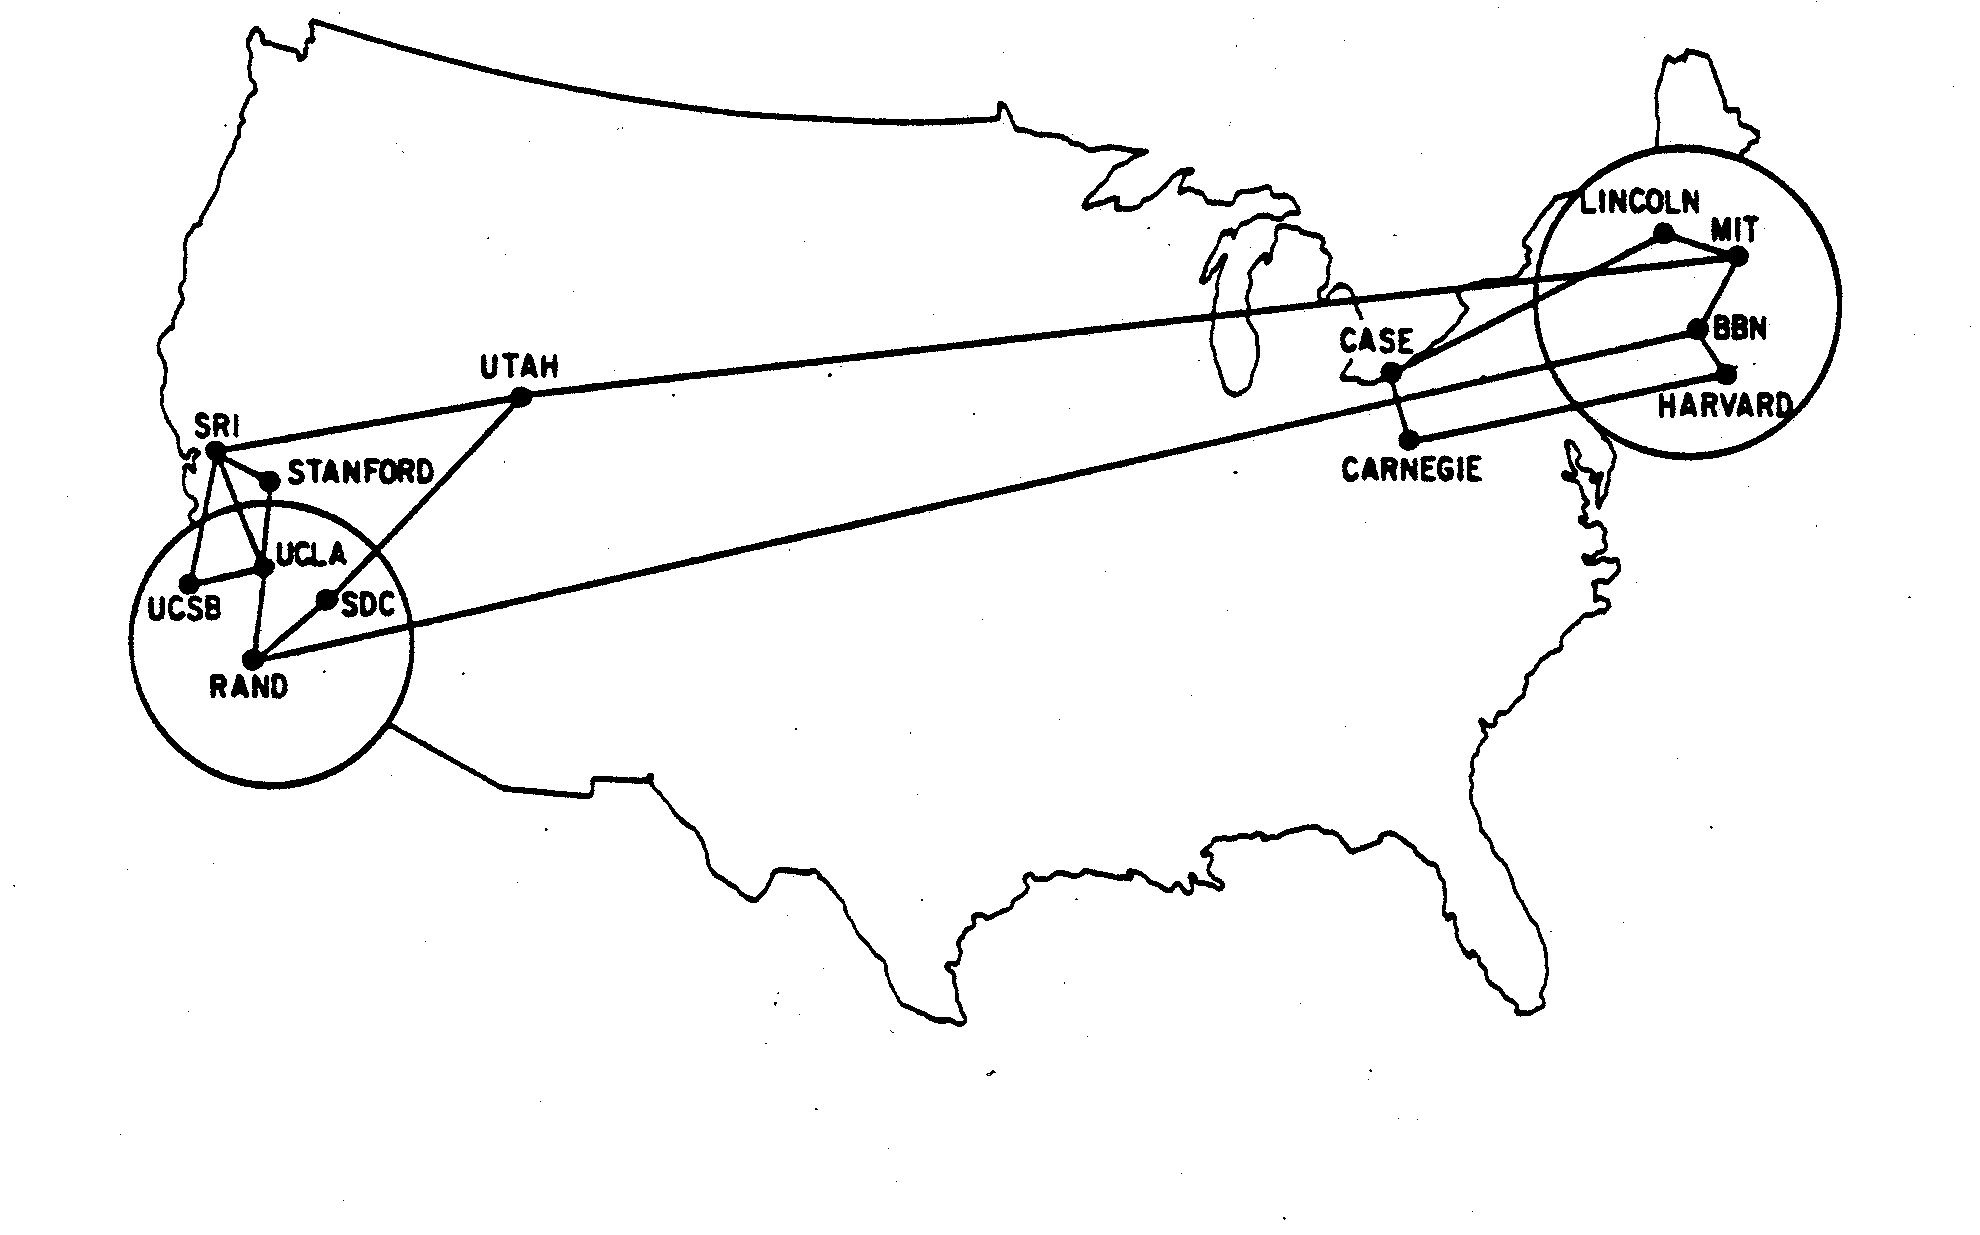
\includegraphics[width=0.7\textwidth]{./images/f7dec1970.jpg}
    \caption{
        The Internet (more precisely, ARPANET) in December 1970.
        Nodes are computers, connected by a link if they can directly communicate with each other.
        At the time, only 13 computers participated in that network.
    }
\end{figure}

\begin{code}
\begin{minted}[linenos, breaklines, frame=single]{text}
UCSB SRI UCLA
SRI UCLA STAN UTAH
UCLA STAN RAND
UTAH SDC MIT
RAND SDC BBN
MIT BBN LINC
BBN HARV
LINC CASE
HARV CARN
CASE CARN
\end{minted}
\caption{\texttt{arpa.adj}}
\end{code}

The following \textbf{diagram}, built from the adjacencies in \verb|arpa.adj|, contains the same information as in the above figure, without the distracting details of US geography;
this is actually an important point, as networks only reflect the \textbf{topology} of the object being studied.

\begin{code}
\begin{minted}[linenos, breaklines, frame=single]{python}
H = nx.read_adjlist("../data/arpa.adj")
opts = { "with_labels": True, "node_color": 'y' }
nx.draw(H, **opts)
\end{minted}
\caption{\texttt{arpa.adj}}
\end{code}

\begin{figure}[H]
    \centering
    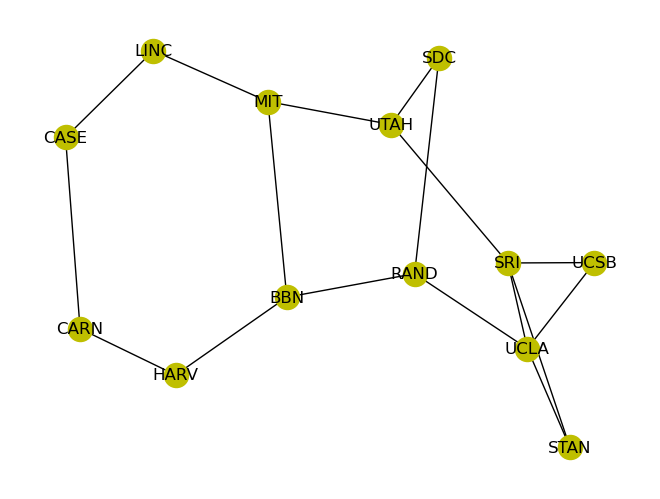
\includegraphics[width=0.7\textwidth]{./images/qwe_download.png}
    \caption{ The ARPA Network as a Graph }
\end{figure}

\subsection{Simple Graphs}
A \textbf{simple graph} is a pair $G = (X,E)$ consisting of a finite set $X$ of objects called \textit{nodes}, \textit{vertices}, or \textit{points} and a set of \textit{links} or \textit{edges} $E$ which are each a set of two different vertices. 
\begin{itemize}
    \item   We can also write $E \subseteq \binom{X}{2}$, where $\binom{X}{2}$ ($X$ \textit{choose} 2) is the set of all $2$-element subsets of $X$.
    \item   The \textbf{order} of the graph $G$ is denoted as $n = |X|$, where $n$ is the number of vertices in the graph.
    \item   The \textbf{size} of the graph is denoted as $m = |E|$, where $m$ is the number of edges in the graph.
            Naturally, $m \leq \binom{n}{2}$.
\end{itemize}

\subsection{Subgraphs \& Induced Subgraphs}
Given $G = (X,E)$, a \textbf{subgraph} of $G$ is $H=(Y, E_H)$ with $Y \subseteq X$ and $E_H \subseteq  E \cap \binom{Y}{s}$;
therefore, all the nodes in $H$ are also in $G$ and any edge in $H$ was also in $G$, and is incident only to vertices in $Y$.
\\\\
One of the most important subgraphs of $G$ is the \textbf{induced subgraph} on $Y \subseteq X$: $H = (Y, E \cap \binom{Y}{2})$;
that is, given a subset $Y$ of $X$, we include all possible edges from the original graph $G$ too.
Each node has a list of \textbf{neighbours} which are the nodes it is directly connected to by an edge of the graph.

\subsection{Important Graphs}
The \textbf{complete graph} on a vertex set $X$ is the graph with edge set $\binom{X}{2}$.
For example, if $X = \{0,1,2,3 \}$, then $E = \{01,02,03,12,13,23\}$
\\\\
The \textbf{Petersen graph} is a graph on 10 vertices with 15 edges.
It can be constructed as the complement of the line graph of the complete graph $K_5$, that is, as the graph with the vertex set $X = \binom{ \{0,1,2,3,4\} }{2}$ (the edge set of $K_5$) and with an edge between $x,y \in X$ whenever $x \cap y = \emptyset$.
\\\\
A graph is \textbf{bipartite} if we can divide the node set $X$ into two subsets $X_1$ and $X_2$ such that:
\begin{itemize}
    \item   $X_1 \cap X_2 = \emptyset$  (the sets have no edge in common);
    \item   $X_1 \cup X_2 = X$.
\end{itemize}

For any edge $(u_1, u_2)$, we have $u_1 \in X_1$ and $u_2 \in X_2$; that is, we only ever have edges between nodes from different sets.
Such graphs are very common in Network Science, where nodes in the network represent two different types of entities; for example, we might have a graph wherein nodes represent students and modules, with edges between students and modules they were enrolled in, often called an \textbf{affiliation network}.
\\\\
A \textbf{complete bipartite graph} is a particular bipartite graph wherein there is an edge between every node in $X_1$ and every node in $X_2$.
Such graphs are denoted $K_{m,n}$, where $|X_1| = m$ and $|X_2|=n$.
\\\\
The \textbf{path graph} with $n$ nodes, denoted $P_n$, is a graph where two nodes have degree 1, and the other $n-2$ have degree 2.
\\\\
The \textbf{cycle graph} on $n \geq 3$ nodes, denoted $C_n$ (slightly informally) is formed by adding an edge between the two nodes of degree 1 in a path graph.

\subsection{New Graphs from Old}
The \textbf{complement} of a graph $G$ is a graph $H$ with the same nodes as $G$ but each pair of nodes in $H$ are adjacent if and only if they are \textit{not adjacent} in $G$.
The complement of a complete graph is an empty graph.
\\\\
A graph $G$ can be thought of as being made from ``things'' that have connection to each other: the ``things'' are nodes, and their connections are represented by an edge.
However, we can also think of edges as ``things'' that are connected to any other edge with which they share a vertex in common.
This leads to the idea of a line graph:
the \textbf{line graph} of a graph $G$, denoted $L(G)$ is the graph where every node in $L(G)$ corresponds to an edge in $G$, and for every pair of edges in $G$ that share a node, $L(G)$ has an edge between their corresponding nodes.

\section{Matrices of Graphs}
There are various was to represent a graph, including the node set, the edge set, or a drawing of the graph;
one of the most useful representations of a graph for computational purposes is as a \textbf{matrix}; the three most important matrix representations are:
\begin{itemize}
    \item   The \textbf{adjacency matrix} (most important);
    \item   The \textbf{incidence matrix} (has its uses);
    \item   The \textbf{graph Laplacian} (the coolest).
\end{itemize}

\subsection{Adjacency Matrices}
The \textbf{adjacency matrix} of a graph $G$ of order $n$ is a square $n \times n$ matrix $A = (a_{i,j})$ with rows \& columns corresponding to the nodes of the graph, that is, we number the nodes $1, 2, \dots, n$.
Then, $A$ is given by:
\begin{align*}
    a_{i,j} =
    \begin{cases}
        1 & \text{if nodes } i \text{ and } j \text{ are joined by an edge,} \\
        0 & \text{otherwise}
    \end{cases}
\end{align*}

Put another way, $a_{i,j}$ is the number of edges between node $i$ and node $j$.
Properties of adjacency matrices include:
\begin{itemize}
    \item   $\sum^N_{i=1} \sum^N_{j=1} a_{i,j} = \sum_{u \in X}\text{deg}(u)$ where $\text{deg}(u)$ is the degree of $u$.
    \item   All graphs that we've seen hitherto are \textit{undirected}: for all such graphs, $A$ is symmetric.
            $A = A^T$ and, equivalently, $a_{i,j} = a{j,i}$.
    \item   $a_{i,i} = 0$ for all $i$.
    \item   In real-world examples, $A$ is usually \textbf{sparse} which means that $\sum^N_{i=1} \sum^N_{j=1} a_{i,j} \ll n^2$, that is, the vast majority of the entries are zero.
            Sparse matrices have huge importance in computational linear algebra: an important idea is that is much more efficient to just store the location of the non-zero entities in a sparse matrix.
\end{itemize}

Any matrix $M = (m_{i,j})$ with the properties that all entries are zero or one and that the diagonal entries are zero (i.e., $m_{i,j}=0$) is an adjacency matrix of \textit{some} graph (as long as we don't mind too much about node labels).
In a sense, every square matrix defines a graph if:
\begin{itemize}
    \item   We allow loops (an edge between a node and itself).
    \item   Every edge has a weight: this is equivalent to the case for our more typical graphs that every potential edge is weighted 0 (is not in the edge set)  or 1 (is in the edge set).
    \item    There are two edges between each node (one in each direction) and they can have different weights.
\end{itemize}

\subsubsection{Examples of Adjacency Matrices}
Let $G = G(X,E)$ be the graph with $X = \{a,b,c,d,e\}$ nodes and edges $\{a \leftrightarrow b, b \leftrightarrow c, b \leftrightarrow d, c \leftrightarrow d, d \leftrightarrow e \}$.
Then:
\begin{align*}
    A =
    \begin{pmatrix}
        0 & 1 & 0 & 0 & 0 \\
        1 & 0 & 1 & 1 & 0 \\
        0 & 1 & 0 & 1 & 0 \\
        0 & 1 & 1 & 0 & 1 \\
        0 & 0 & 0 & 1 & 0 \\
    \end{pmatrix}
\end{align*}

The adjacency matrix of $K_4$ is:
\begin{align*}
    A =
    \begin{pmatrix}
        0 & 1 & 1 & 1 \\
        1 & 0 & 1 & 1 \\
        1 & 1 & 0 & 1 \\
        1 & 1 & 1 & 0 \\
    \end{pmatrix}
\end{align*}

\subsection{Degree}
The \textbf{degree} of a node in a simple graph is the number of nodes to which it is adjacent, i.e., its number of neighbours.
For a node $v$ we denote this number $\text{deg}(v)$.
The degree of a node can serve as a (simple) measure of the importance of a node in a network.
Recall that one of the basic properties of an adjacency matrix is $\sum^n_{i=1} \sum^n_{j=1} a_{i,j} = \sum_{u \in X} \text{deg}(u)$, where $\text{deg}(u)$ is the degree of $u$ and $n$ is the order of the graph;
this relates to a (crude) measure of how connected a network is: the \textbf{average degree}:
\begin{align*}
    \text{Average degree} = \frac{1}{n} \sum_{u \in X} \text{deg}(u) = \frac{1}{n}\sum^n_{i,j} a_{i,j}
\end{align*}
However, if the size of the network (the number of edges) is $m$, then the total sum of degrees is $2m$ (since each edge contributes to the degree count of two nodes), meaning that the average degree is $\frac{2m}{n}$.

\subsection{Walks}
A \textbf{walk} in a graph is a series of edges (perhaps with some repeated) $\{ u_1 \leftrightarrow v_1, u_2 \leftrightarrow u_2, \dots, u_p \leftrightarrow v_p\}$ with the property that $v_i = u_{i+1}$.
If $v_p = u_1$, then it is a \textbf{closed walk}.
The \textbf{length} of a walk is the number of edges in it.
\\\\
Adjacency matrices can be used to enumerate the number of walks of a given length between a pair of vertices.
Obviously, $a_{i,j}$ is the number of walks of length 1 between node $i$ and node $j$.
We can extract that information for node $j$ by computing the product of $A$ and $e_j$ (column $j$of the identity matrix).

\section{Connectivity \& Permutations}
\subsection{Notation}
To start, let's decide on our notation:
\begin{itemize}
    \item   If we write $A = (a_{i,j})$, we mean that $A$ is a matrix and $a_{i,j}$ is its entry row $i$, column $j$.
    \item   We also write such entries as $(A)_{i,j}$;
            the reason for this slightly different notation is to allow us to write, for example, $(A^2)_{i,j}$ is the entry in row $i$, column $j$ of $B = A^2$.
    \item   The \textbf{trace} of a matrix is the sum of its diagonal entries, that is, $\text{tr}(A) = \sum^n_{i=1}a_{i,i}$. (Very standard).
    \item   When we write $A > 0$, we mean that all entries of $A$ are positive.
\end{itemize}

\subsection{Counting Walks}
Recall that the \textbf{adjacency matrix} of a graph $G$ of order $N$ is a square $n \times n$ matrix $A = (a_{i,j})$ with rows and columns corresponding to the nodes of the graph.
$a_{i,j}$ is set to be the number of edges between nodes $i$ and $j$.
We learned previously that:
\begin{itemize}
    \item   If $e_j$ is the $j^\text{th}$ column of the identity matrix $I_n$, then $(Ae_j)_i$ is the number of walks of length 1 from node $i$ to node $j$.
            Also, it is the same as $a_{i,j}$.

    \item   Moreover, $(A(Ae_j))_i = (A^2e_j)$ is the number of walks of length 2 from node $i$ to node $j$.
            We can conclude that, if $B=A^2$, then $b_{i,j}$ is the number of walks of length 2 between nodes $i$ and $j$.
            Note that $b_{i,i}$ is the degree of node $i$.

    \item   In fact, if $B=A^k$, then $b_{i,j}$ is the number of walks of length $k$ between nodes $i$ and $j$.
\end{itemize}

\subsection{Paths}
A \textbf{trail} is  walk with no repeated edges.
A \textbf{cycle} is a trail in which the first and last nodes are the same, but no other node is repeated;
a \textbf{triangle} is a cycle of length 3.
A \textbf{path} is a walk in which no nodes (and so no edges) are repeated.
(The idea of a path is hugely important in network theory, and we will return to it often).
\\\\
The \textbf{length} of a path is the number of edges in that path.
A path from node $u$ to node $v$ is a \textbf{shortest path} if there is no path between them that is shorter (although there could be other paths of the same length).
Finding shortest paths in a network is a major topic that we will return to at another time.
\begin{itemize}
    \item   Every path is also a walk.
    \item   If a particular walk is the shortest walk between two nodes then it is also the shortest path between two nodes.
    \item   If $k$ is the smallest natural number of which $(A^k)_{i,j} \neq 0$, then the shortest walk from node $i$ to node $j$ is of length $k$.
    \item   It follows that $k$ is also the length of the shortest path from node $i$ to node $j$.
\end{itemize}

For example, consider the following adjacency matrix and its powers:
\begin{align*}
A =
\begin{pmatrix}
    0 & 1 & 0 & 0 & 0 \\
    1 & 0 & 1 & 0 & 0 \\
    0 & 1 & 0 & 1 & 1 \\
    0 & 0 & 1 & 0 & 1 \\
    0 & 0 & 1 & 1 & 0
\end{pmatrix}
\end{align*}

\begin{align*}
A^2 =
\begin{pmatrix}
    1 & 0 & 1 & 0 & 0 \\
    0 & 2 & 0 & 1 & 1 \\
    1 & 0 & 3 & 0 & 0 \\
    0 & 1 & 1 & 2 & 1 \\
    0 & 1 & 1 & 1 & 2
\end{pmatrix}
\end{align*}

\begin{align*}
A^3 =
\begin{pmatrix}
    0 & 2 & 0 & 1 & 1 \\
    2 & 0 & 4 & 1 & 1 \\
    0 & 4 & 2 & 4 & 4 \\
    1 & 1 & 4 & 2 & 3 \\
    1 & 1 & 4 & 3 & 2
\end{pmatrix}
\end{align*}

We can observe that, where $A$ is the adjacency matrix of the graph $G$:
\begin{itemize}
    \item   $(A^2)_{i,i}$ is the degree of node $i$.
    \item   $\text{tr}(A^2)$ is the degree sum of the nodes in $G$.
    \item   $(A^3)_{i,i} \neq 0 $ if node $i$ is in a triangle.
    \item   $\frac{\text{tr}(A^3)}{6}$ is the number of triangles in $G$.
    \item   If $G$ is bipartite, then $(A^3)_{i,j} = 0$ for all $i,j$.
\end{itemize}

\subsection{Connectivity}
Let $G$ be a graph and $A$ its adjacency matrix:
in $G$, node $i$ can be \textbf{reached} from node $j$ if there is a path between them.
If node $i$ is reachable from node $j$, then $(A^k)_{i,j} \neq 0$ for some $k$.
Also, note that $k \leq n$.
Equivalently, since each power of $A$ is non-negative, we can say that $(I + A + A^2 + A^3 + \cdots + A^k) > 0$.
\\\\
A graph/network is \textbf{connected} if there is a path between every pair of nodes.
That is, every node is reachable from every other node.
If a graph is not connected, we say that it is \textbf{disconnected}.
Determining if a graph is connected or not is important; we'll see later that this is especially important with directed graphs.
A graph $G$ of order $n$ is connected if and only if, for each $i,j$, there is some $K \leq n$ for which $(A^k)_{i,j} \neq 0$.

\subsection{Permutation Matrices}
We know that the structure of a network is not changed by labelling its nodes.
Sometimes, it is useful to re-label the nodes in order to expose certain properties, such as connectivity.
Since we think of the nodes as all being numbered from 1 to $n$, this is the same as \textbf{permuting} the numbers of some subset of the nodes.

\begin{figure}[H]
    \centering
    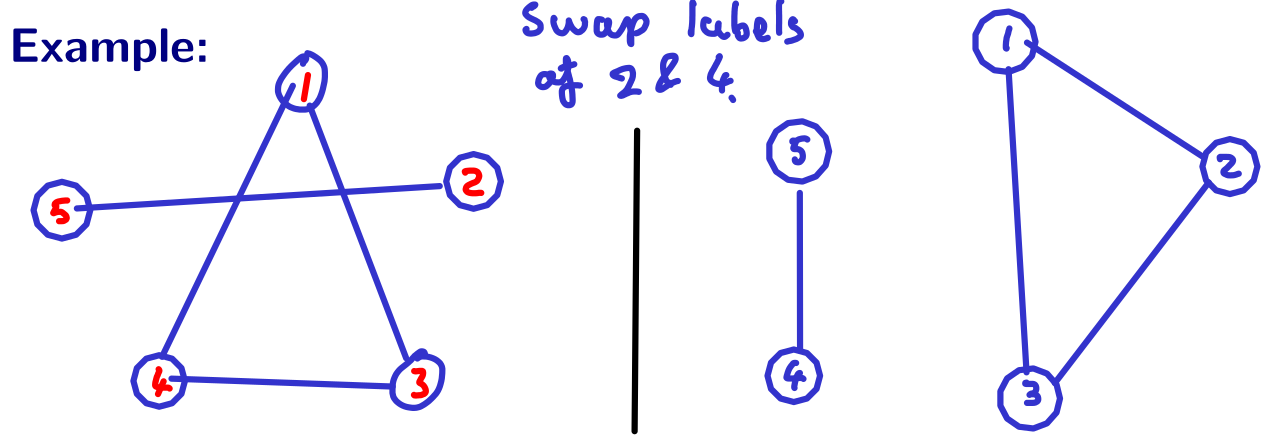
\includegraphics[width=0.7\textwidth]{./images/permexampe.png}
    \caption{ Example wherein nodes are re-labelled to expose certain properties of the graph }
\end{figure}

When working with the adjacency matrix of a graph, such a permutation is expressed in terms of a \textbf{permutation matrix} $P$;
this is a $0$-$1$ matrix (also known as a Boolean or a binary matrix) where this is a single $1$ in every row \& column.
If the nodes of a graph $G$ (with adjacency matrix $A$) are listed as entries in a vector ${q}$, then:
\begin{itemize}
    \item   $Pq$ is a permutation of the nodes.
    \item   $PAP^T$ is the adjacency matrix of the graph with that node permutation applied.
\end{itemize}

In many examples, we will have a symmetric $P$ for the sake of simplicity, but in general, $P \ neq P^T$.
However, $P^TAP = PAP^T$and $P^T = P^{-1}$ so $PAP^T = PAP^{-1}$.
\\\\
A graph with adjacency matrix $A$ is \textbf{disconnected} if and only if there is a permutation matrix $P$ such that
\begin{align*}
A &= P \begin{pmatrix} X & O \\ O^T & Y \end{pmatrix} &
PAP^T &= P \begin{pmatrix} X & O \\ O & Y \end{pmatrix}
\end{align*}
where $O$ represents the zero matrix with the same number of rows as $X$ and the same number of columns as $Y$.

\section{Permutations \& Bipartite Networks}
\subsection{Graph Connectivity}
Recall that a graph is \textbf{connected} if there is a path between every pair of nodes.
If the graph is not connected, we say that it is \textbf{disconnected}.
We now know how to check if a graph is connected by looking at powers of its adjacency matrix.
However, that is not very practical for large networks.
Instead, we can determine if a graph is connected by just looking at the adjacency matrix, provided that we have ordered the nodes properly.

\subsection{Connected Components}
If a network is not connected, then we can divide it into \textbf{components} which \textit{are} connected.
The number of connected components is the number of blocks in the permuted adjacency matrix.

\begin{figure}[H]
    \centering
    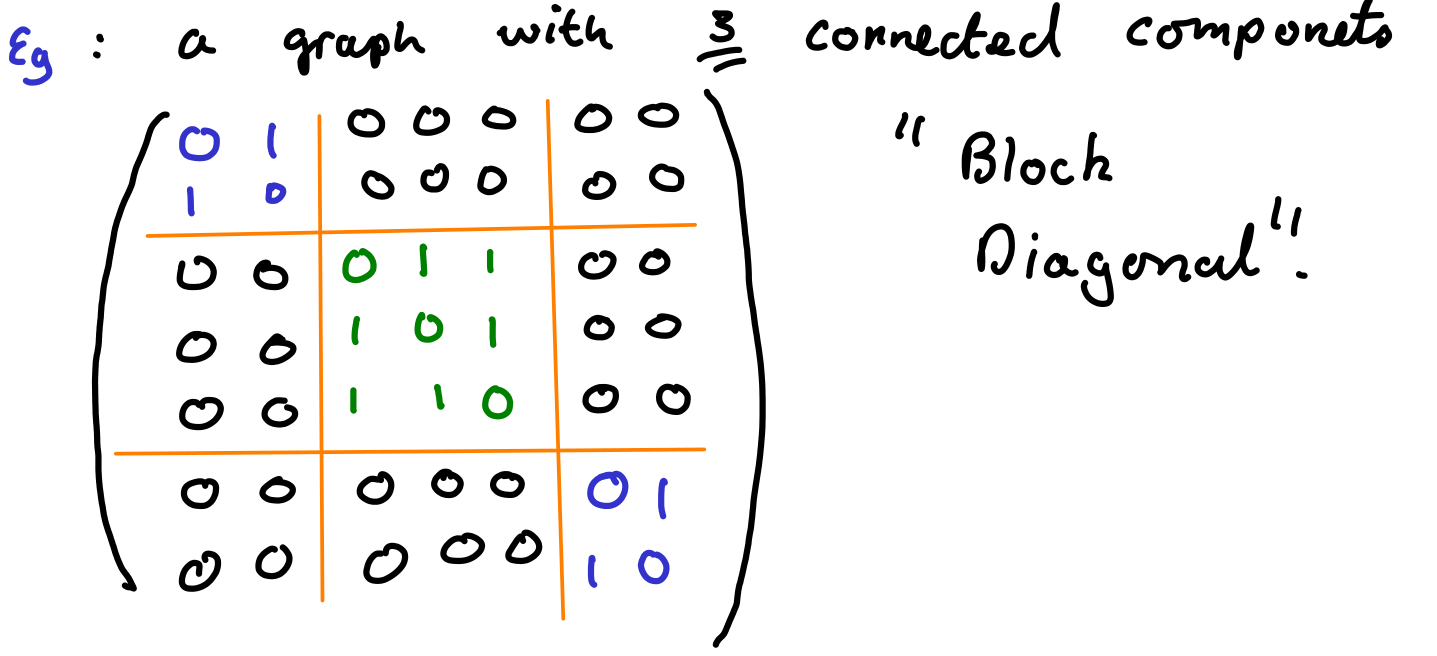
\includegraphics[width=0.7\textwidth]{./images/connectedcomponents.png}
    \caption{ Connected components example }
\end{figure}

\section{Bipartite Networks: Colours \& Computations}
\subsection{Class Survey Example}
\begin{figure}[H]
    \centering
    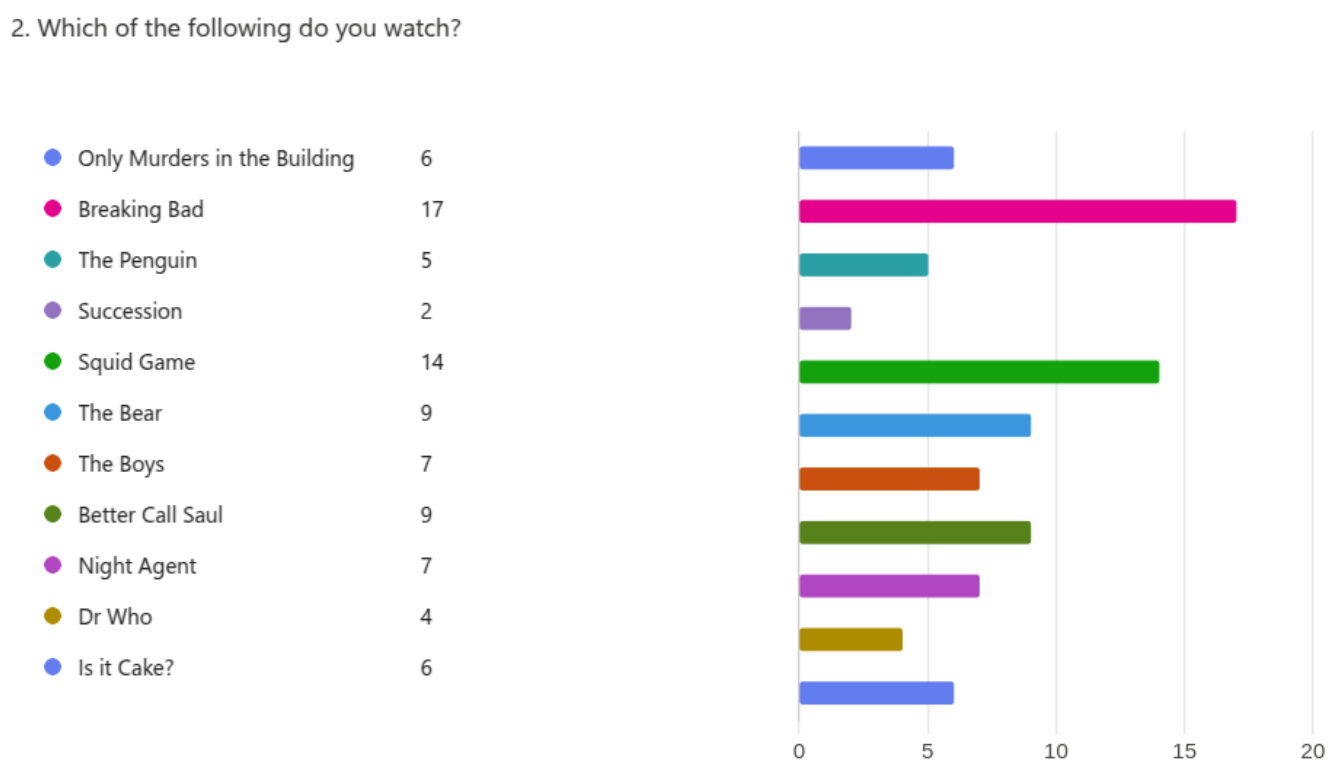
\includegraphics[width=0.7\textwidth]{./images/suverydata.png}
    \caption{ Final survey data }
\end{figure}

\begin{figure}[H]
    \centering
    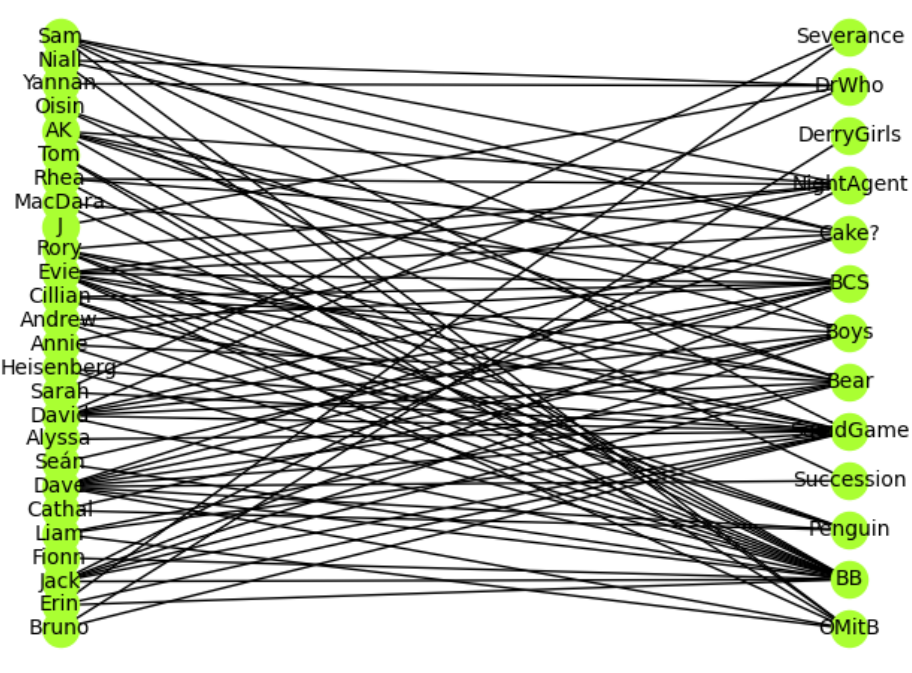
\includegraphics[width=0.7\textwidth]{./images/suverygaaph.png}
    \caption{ Final survey graph, with order 39 and size 87 }
\end{figure}

\begin{figure}[H]
    \centering
    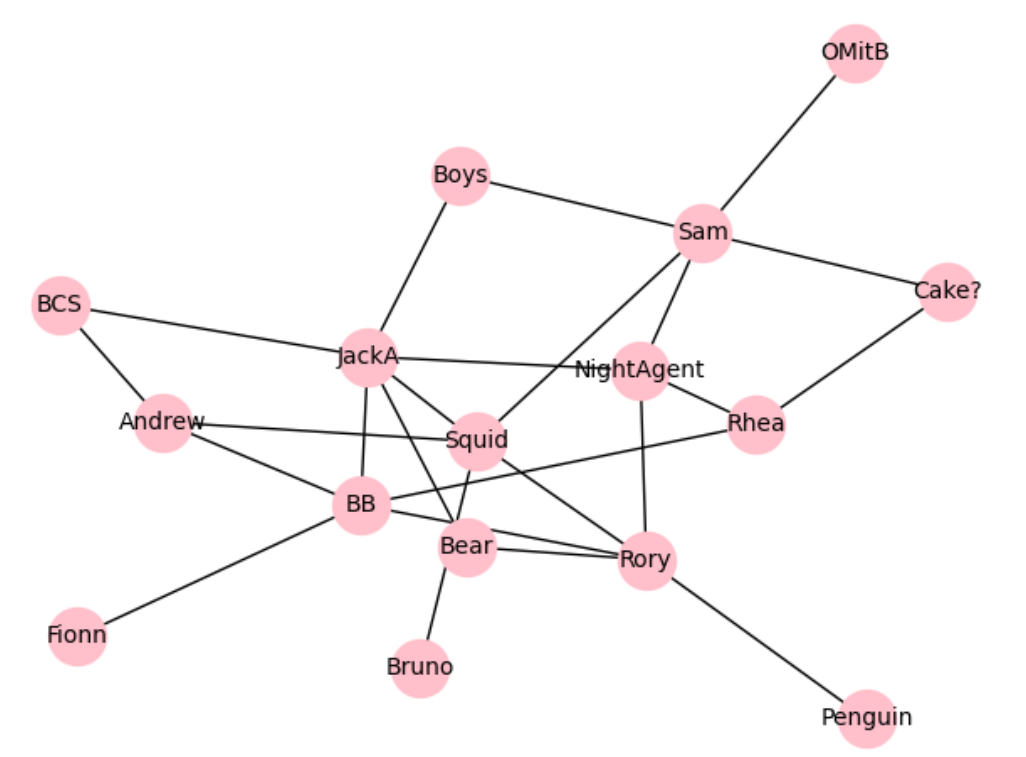
\includegraphics[width=0.7\textwidth]{./images/surveysubgrap.png}
    \caption{ Subgraph of the survey network based on 7 randomly chosen people, with order 16 and size 24 }
\end{figure}

\begin{figure}[H]
    \centering
    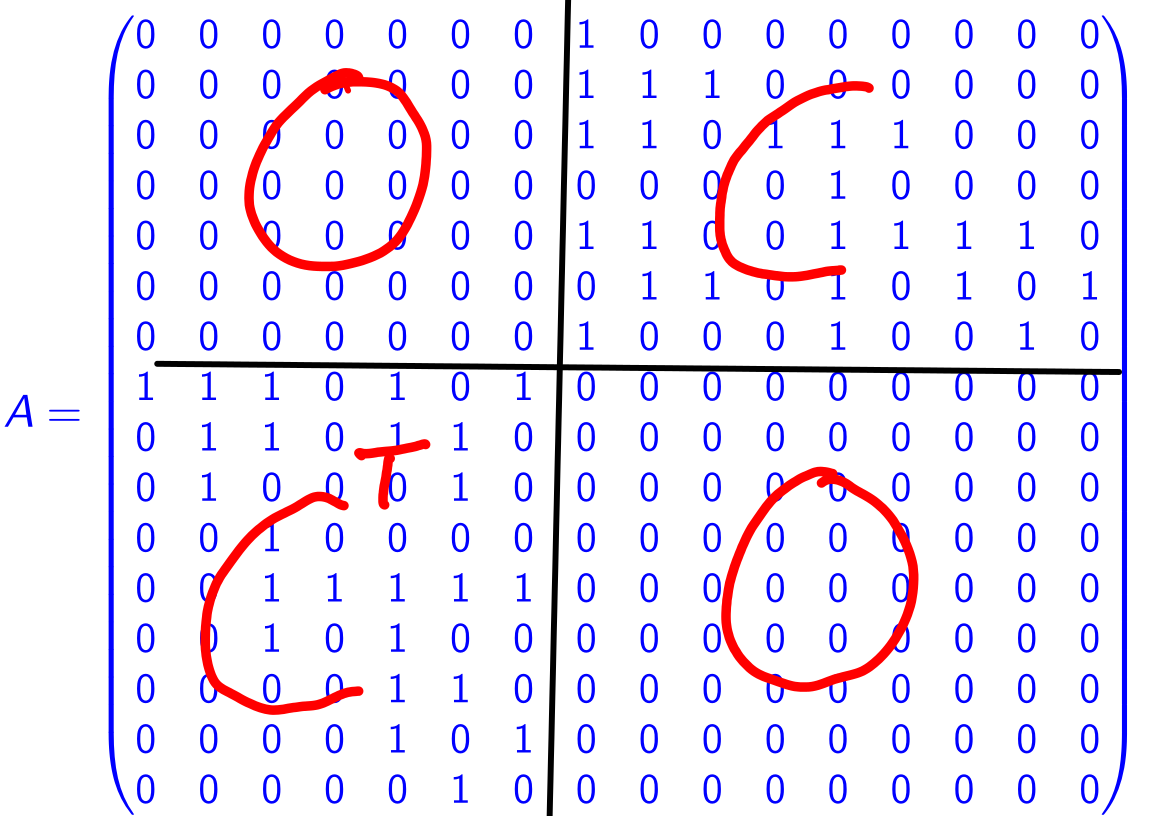
\includegraphics[width=0.7\textwidth]{./images/surveymatrix.png}
    \caption{ Adjacency matrix where the nodes for people are listed first }
\end{figure}

\begin{figure}[H]
    \centering
    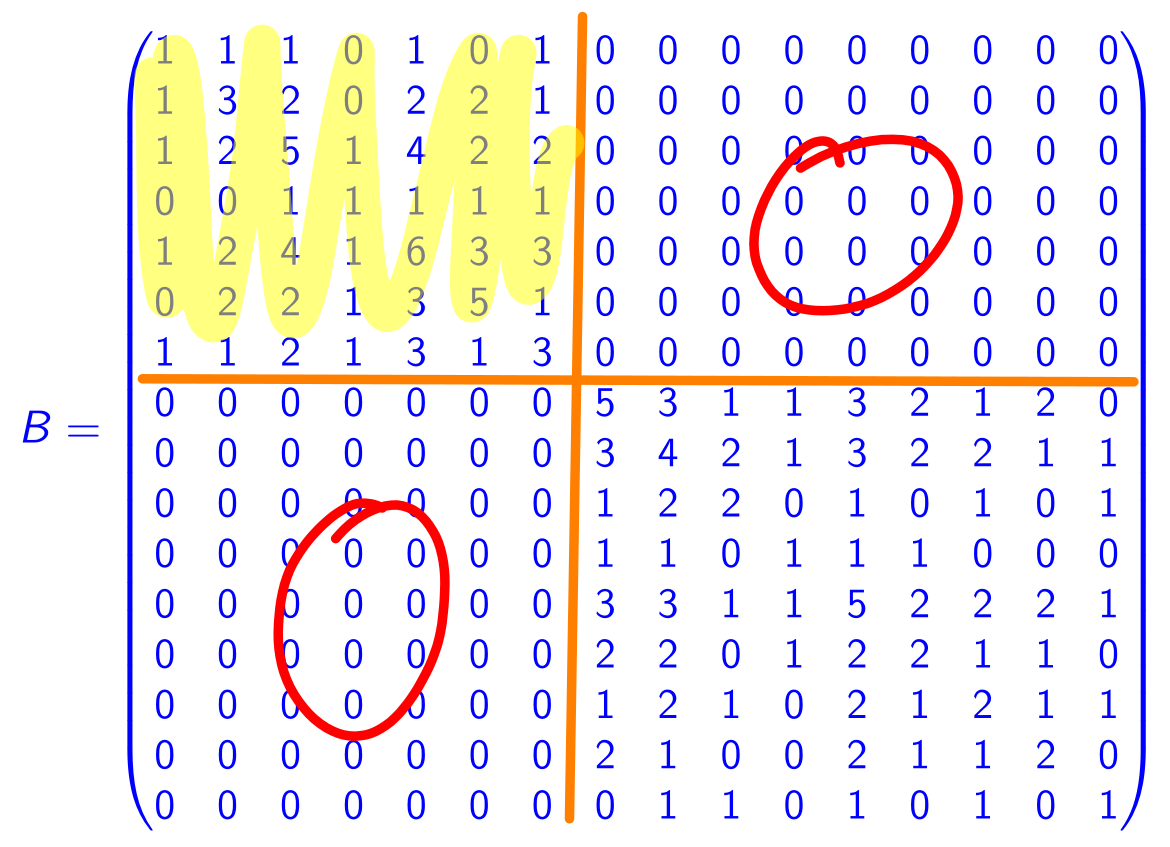
\includegraphics[width=0.7\textwidth]{./images/surveymatrix2.png}
    \caption{ $B = A^2$ }
\end{figure}

Since we know from before that $(A^k)_{i,j}$ is the number of walks of length $k$between nodes $i$ and $j$, we can see that in this context:
\begin{itemize}
    \item   For the first 7 rows \& columns, $b_{i,j}$ is the number of programmes in common between person $i$ and person $j$.
            (This even works for $i=j$, but the number of programmes a person has in common with themselves is just the number they watch).
    \item   For the last 9 rows \& columns, $b_{i,j}$ is the number of people who watch both programmes $i$ and $j$.
\end{itemize}

\subsection{Projections}
Given a bipartite graph $G$ whose node set $V$ has parts $V_1$ \& $V_2$, and \textbf{projection} of $G$ onto (for example) $V_1$ is the graph with:
\begin{itemize}
    \item   Node set $V_1$;
    \item   An edge between a pair of nodes in $V_1$ if they share a common neighbour in $G$.
\end{itemize}

In the context of our survey example, a projection onto $V_1$ (people/actors) gives us the graph of people who share a common programme.
To make such a graph:
\begin{itemize}
    \item   Let $A$ be the adjacency matrix of $G$.
    \item   Let $B$ be the submatrix of $A^2$ associated with the nodes in $V_1$.
    \item   Let $C$ be the adjacency matrix with the property:
            \begin{align*}
                c_{i,j} =
                \begin{cases}
                    1 & b_{i,j} > 0 \text{ and } i \neq j \\
                    0 & \text{otherwise}
                \end{cases}
            \end{align*}
            That is, $b_{i,j} = 0 $ or $i=j$.
    \item   Let $G_{V_1}$ be the graph on $V_1$ with adjacency matrix $C$.
            Then, $G_{V_1}$ is the \textbf{projection of $G$ onto $V_1$}.
\end{itemize}

\begin{figure}[H]
    \centering
    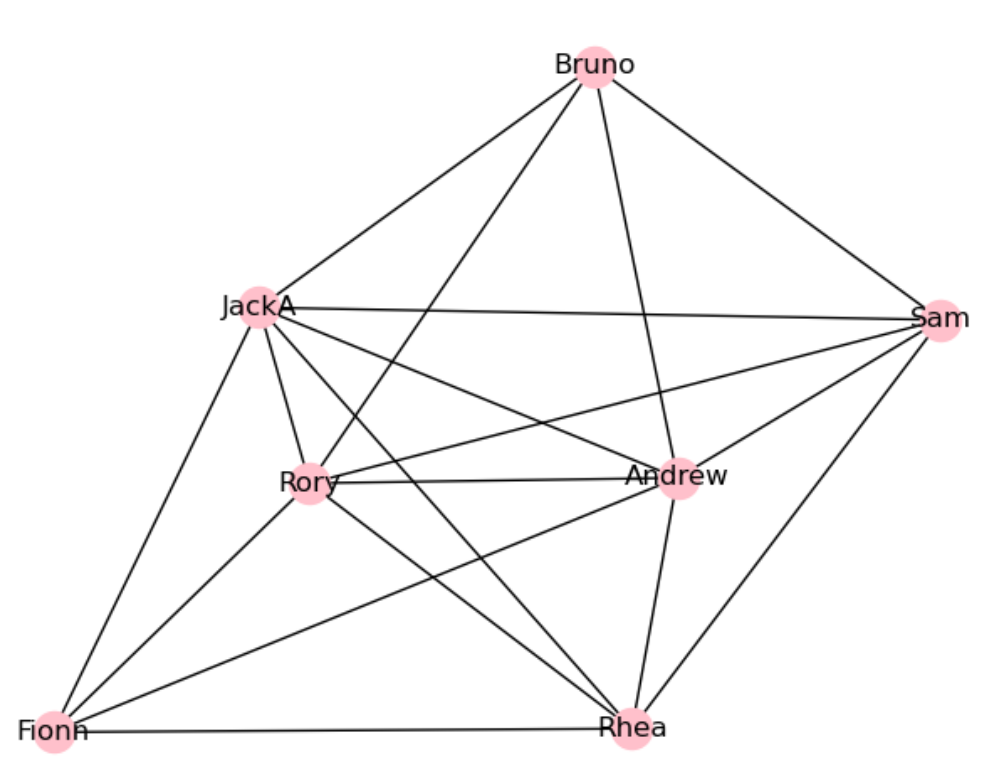
\includegraphics[width=0.7\textwidth]{./images/surveygv1.png}
    \caption{ $G_{V_1}$ computed for our survey data }
\end{figure}

\subsection{Colouring}
\begin{figure}[H]
    \centering
    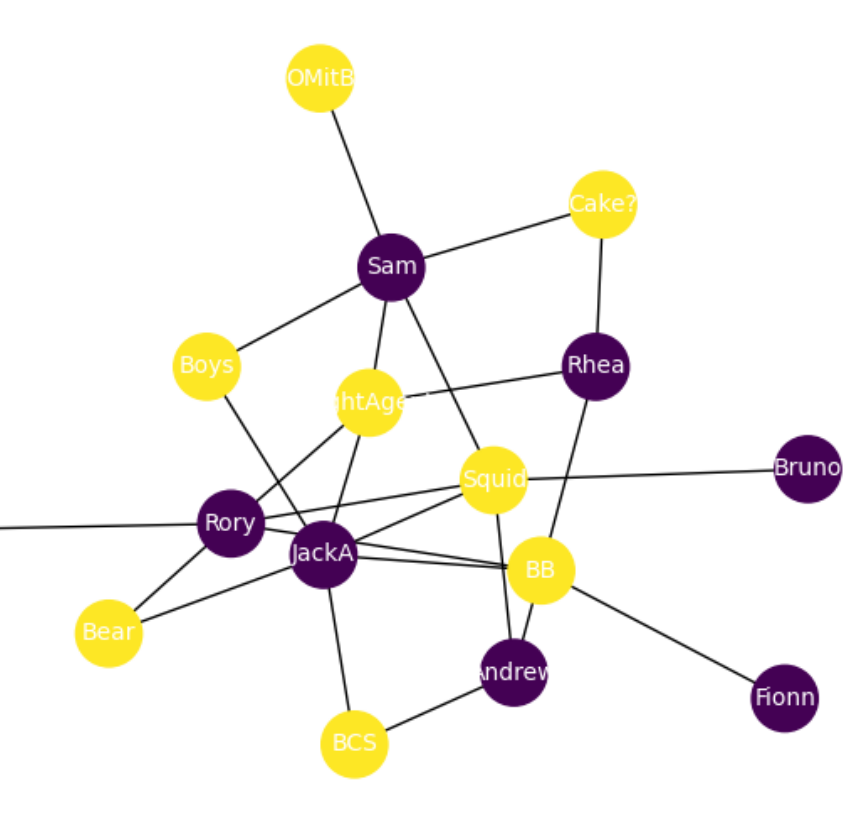
\includegraphics[width=0.7\textwidth]{./images/colouredsurvey.png}
    \caption{ The original survey graph is more easily digestible if coloured }
\end{figure}

For any bipartite graph, we can think of the nodes in the two sets as \textbf{coloured} with different colours.
For instance, we can think of nodes in $X_1$ as white nodes and those in $X_2$ as black nodes.
A \textbf{vertex-colouring} of a graph $G$is an assignment of (finitely many) colours to the nodes of $G$ such that any two nodes which are connected by an edge have different colours.
A graph is called \textbf{$N$-colourable} if it has a vertex colouring with at most $N$ colours.
The \textbf{chromatic number} of a graph $G$ is the \textit{smallest $N$} for which a graph $G$ is $N$-colourable.
The following statements about a graph $G$ are equivalent:
\begin{itemize}
    \item   $G$ is bipartite;
    \item   $G$ is 2-colourable;
    \item   Each cycle in $G$ has even length.
\end{itemize}

\section{Trees}
A \textbf{cycle} in a simple graph provides, for any two nodes on that cycle, at least two different paths from node $a$ to node $b$.
It can be useful to provide alternative routes for connectivity in case one of the edges should fail, e.g., in an electrical network.
\\\\
A graph is called \textbf{acyclic} if it does not contain any cycles.
A \textbf{tree} is a simple graph that is \textit{connected} \& \textit{acyclic}.
In other words, between any two vertices in a tree there is exactly one simple path.
Trees can be characterised in many different ways.
\\\\
\textbf{Theorem:} Let $G=(X,E)$ be a (simple) graph of order $n=|X|$ and size $m=|E|$.
Then, the following are equivalent:
\begin{itemize}
    \item   $G$ is a tree (i.e., acyclic \& connected);
    \item   $G$ is connected and $m=n-1$.
    \item   $G$ is a minimally connected graph (i.e., removing any edge will disconnect $G$).
    \item   $G$ is acyclic and $m=n-1$.
    \item   $G$ is a maximally acyclic graph (i.e., adding any edge will introduce a cycle in $G$);
    \item   There is a unique path between each pair of nodes in $G$.
\end{itemize}

All trees are \textbf{bipartite}:
there are a few ways of thinking about this;
one is that a graph is bipartite if it has no cycles of odd length -- since a tree has no cycles, it must be bipartite.

\subsection{Cayley's Formula}
\textbf{Theorem:} there are exactly $n^{n-2}$ distinct (labelled) trees on the $n$-element vertex set $X=\{0,1,2, \dots, n-1\}$ if $n>1$.

\subsubsection{Pr\"ufer Codes}
The \textbf{Pr\"fer code} of a tree can be determined (destructively) as follows:
\begin{enumerate}
    \item   Start with a tree $T$ with nodes labelled $0, 1, \dots, n-1$ and an empty list $a$.
    \item   Find the \textbf{leaf node} $x$ with the smallest label (with a ``leaf node'' being a node of degree 1. Every tree must have at least two leaf nodes).
    \item   Append the label of its unique neighbour $y$to the list $a$.
    \item   Remove $x$ (and the edge $x \leftrightarrow y$) from $T$.
    \item   Repeat steps 2-3 until $T$ has only two ndoes left.
            We now have the code as a list of length $n-2$.
\end{enumerate}

A tree can be re-constructed from its Pr\"ufer code as the degree of a node $x$ is $1$ plus the number of entries $x$ in the Pr\"ufer code of $T$.
A tree can be computed from a Pr\"ufer code $a$ (where the list $a$ is a list of length $n-2$ with all entries numbered $0$ to $n-1$) as follows:
\begin{enumerate}
    \item   Set $G$ to be a graph with node list $[0,1,2, \dots, n-1]$ and no edges yet.
    \item   Compute the list of node degrees $d$ from the code.
    \item   For $k=0,1,\dots, n-2$: 
            \begin{enumerate}[label=\arabic*.]
                \item   Set $y = a[k]$.
                \item   Set $x$to be the node with the smallest degree in $d$.
                \item   Add the edge $(x,y)$ to $G$.
                \item   Set $d[x]=d[x]-1$and $d[y]=d[y]-1$ (that is, decrease the degrees of both $x$ and $y$ by one).
            \end{enumerate}
    \item   Finally, connect the remaining two nodes of degrees 1 by an edge.
\end{enumerate}

Since we know now that there is a bijection between labelled trees and Pr\"ufer codes, we can prove Cayley's theorem easily:
\begin{enumerate}
    \item   A tree with $n$ nodes has a Pr\"ufer code of length $n-2$.
    \item   There are $n$ choices for each entry in the code.
    \item   So, there are $n^{n-2}$ possible codes for a tree with $n$ nodes.
    \item   So, there are $n^{n-2}$ possible trees with $n$ nodes.
\end{enumerate}

\subsection{Graph \& Tree Traversal}
Often, one has to search through a network to check properties of nodes such as to find the node with the largest degree.
For large unstructured networks, this can be challenging;
fortunately, there are simple \& efficient algorithms to achieve this:
\begin{itemize}
    \item   DFS.
    \item   BFS.
\end{itemize}

\subsubsection{Depth-First Search}
\textbf{Depth-first search (DFS)} works by starting at a root node and travelling as far along one of its branches as it can, then returning to the last unexplored branch.
The main data structure needed to implement DFS is a \textbf{stack}, also known as a Last-In-First-Out (LIFO) queue.
Given a rooted tree $T$ with root $x$, to visit all nodes in the tree:
\begin{enumerate}
    \item   Start with an empty stack $S$.
    \item   Push $x$ onto $S$.
    \item   While $S \neq \emptyset$:
            \begin{enumerate}[label=\arabic*.]
                \item   Pop node $y$ from the stack.
                \item   Visit $y$.
                \item   Push $y$'s children onto the stack.
            \end{enumerate}
\end{enumerate}

\subsubsection{Breadth-First Search}
\textbf{Breadth-first search (BFS)} works by starting at a root node and exploring all the neighbouring nodes (on the same level) first.
Next, it searches their neighbours (level 2), etc.
The main data structure needed to implement BFS is a \textbf{queue}, also known as a First-In-First-Out (FIFO) queue. 
Given a rooted tree $T$ with root $x$, to visit all nodes in the tree:
\begin{itemize}
    \item   Start with an empty queue $Q$.
    \item   Push $x$ onto $Q$.
    \item   While $Q \neq \emptyset$:
            \begin{enumerate}[label=\arabic*.]
                \item   Pop node $y$ from $Q$.
                \item   Visit node $y$.
                \item   Push $y$'s children onto $Q$.
            \end{enumerate}
\end{itemize}

Many questions on networks regarding distance \& connectivity can be answered by a versatile strategy involving a subgraph which is a tree and then searching that; such a tree is called \textbf{spanning tree} of the underlying graph.

\subsubsection{Graph Diameter}
A natural problem arising in many practical applications is the following: given a pair of nodes $x,y$, find one or all the paths from $x$ to $y$ with the fewest number of edges possible.
This is a somewhat complex measure on a network (compared to, say, statistics on node degrees) and we will therefore need a more complex procedure, that is, an algorithm, in order to solve such problems systematically.
\\\\
\textbf{Definition:} let $G=(X,E)$ be a simple graph and let $x,y \in X$.
Let $P(x,y)$ be the set of all paths from $x$ to $y$.
Then:
\begin{itemize}
    \item   The \textbf{distance} $d(x,y)$ from $x$ to $y$ is
            \begin{align*}
                d(x,y) = \text{min}\{ l(p) : p \in P(x,y) \},
            \end{align*}
            the shortest possible length of a path from $x$ to $y$, and a \textbf{shortest path} from $x$ to $y$ is a path $p \in P(x,y)$ of length $l(p) = d(x,y)$.

    \item   The \textbf{diameter} $\text{diam}(G)$ of the network $G$ is the length of the longest shortest path between any two nodes:
            \begin{align*}
                \text{diam}(G) = \text{max}\{ l(p) : p \in P(x,y) \}
            \end{align*}
\end{itemize}




\end{document}
